\documentclass[conference]{IEEEtran}

\usepackage{amsmath,amssymb}
\usepackage{tikz}
\usetikzlibrary{positioning, arrows.meta, shapes.geometric, fit, calc, backgrounds, decorations.pathreplacing, patterns}
\usepackage{hyperref}
\usepackage{booktabs}
\usepackage{caption}
\usepackage{float}
\usepackage{graphicx}
\usepackage{xcolor}
\usepackage{cite}
\usepackage{algorithm}
\usepackage{algorithmic}
\usepackage{multirow}

% Brand colors
\definecolor{garnet}{HTML}{73000A}
\definecolor{atlantic}{HTML}{466A9F}
\definecolor{congaree}{HTML}{1F414D}
\definecolor{horseshoe}{HTML}{65780B}
\definecolor{rose}{HTML}{CC2E40}
\definecolor{honeycomb}{HTML}{A49137}
\definecolor{black90}{HTML}{363636}
\definecolor{black70}{HTML}{5C5C5C}
\definecolor{black50}{HTML}{A2A2A2}
\definecolor{black30}{HTML}{C7C7C7}
\definecolor{sandstorm}{HTML}{FFF2E3}

\begin{document}

\title{Extending Plug-and-Play PPO: Algorithm Comparison, Domain Transfer, and Temporal Prompting for SAM Segmentation}

\author{
\IEEEauthorblockN{Jacob Whisenant, Xeerak Muhammed, J.C. Vaught}
\IEEEauthorblockA{CSCE 775: Deep Reinforcement Learning and Search\\
University of South Carolina\\
February 13, 2026}
}

\maketitle

% ============================================================
% INTRODUCTION
% ============================================================
\section{Introduction}

The Segment Anything Model (SAM)~\cite{Kirillov2023SAM} introduced a paradigm shift in image segmentation by enabling prompt-driven, class-agnostic mask prediction across virtually any visual domain. Given a set of input prompts such as points, bounding boxes, or text, SAM produces high-quality segmentation masks without requiring task-specific fine-tuning. However, SAM's performance is highly sensitive to the quality and placement of these prompts. A poorly placed point prompt can yield a mask that captures the wrong region entirely, while a well-placed one produces near-perfect segmentation. This sensitivity creates a critical bottleneck: in automated pipelines where no human operator is available to provide prompts interactively, the segmentation quality depends entirely on the prompt selection strategy.

Liu et al.~\cite{Liu2025PlugAndPlayPPO} recently addressed this bottleneck by formulating prompt optimization as a reinforcement learning problem. Their Plug-and-Play PPO method trains a policy network using Proximal Policy Optimization~\cite{Schulman2017PPO} to iteratively refine point prompt distributions, guided by a dual-space heterogeneous graph encoding constructed from DINOv2~\cite{Oquab2024DINOv2} features. The method achieves state-of-the-art results on several benchmarks, surpassing both manual prompt strategies and prior automated approaches. Despite these advances, several natural extensions remain unexplored. The original work uses only PPO as the RL algorithm, leaving open the question of whether off-policy methods with continuous action spaces might improve sample efficiency. The evaluation is restricted to standard computer vision benchmarks, leaving domain transfer to specialized fields such as medical imaging, remote sensing, and marine perception untested. The method operates on static images, with no adaptation for temporally consistent video segmentation via SAM 2~\cite{Ravi2024SAM2}. The reward function uses standard IoU, without boundary-aware or class-balanced shaping that could improve performance on challenging structures.

We propose to replicate the Plug-and-Play PPO framework and extend it along four axes. First, we replace PPO with Soft Actor-Critic (SAC)~\cite{Haarnoja2018SAC} and Twin Delayed DDPG (TD3)~\cite{Fujimoto2018TD3} to compare on-policy versus off-policy learning for prompt optimization. Second, we evaluate domain transfer to medical polyp segmentation (KVASIR-SEG~\cite{Jha2020KvasirSEG}) and remote sensing imagery~\cite{Osco2023SAMRemoteSensing}. Third, we adapt the prompt optimizer for SAM 2 video segmentation with temporal consistency constraints. Fourth, we introduce boundary-weighted reward shaping~\cite{Ng1999RewardShaping} to improve mask quality on thin and irregular structures.

% ============================================================
% FIGURE 1: SYSTEM ARCHITECTURE
% ============================================================
\begin{figure*}[t]
\centering
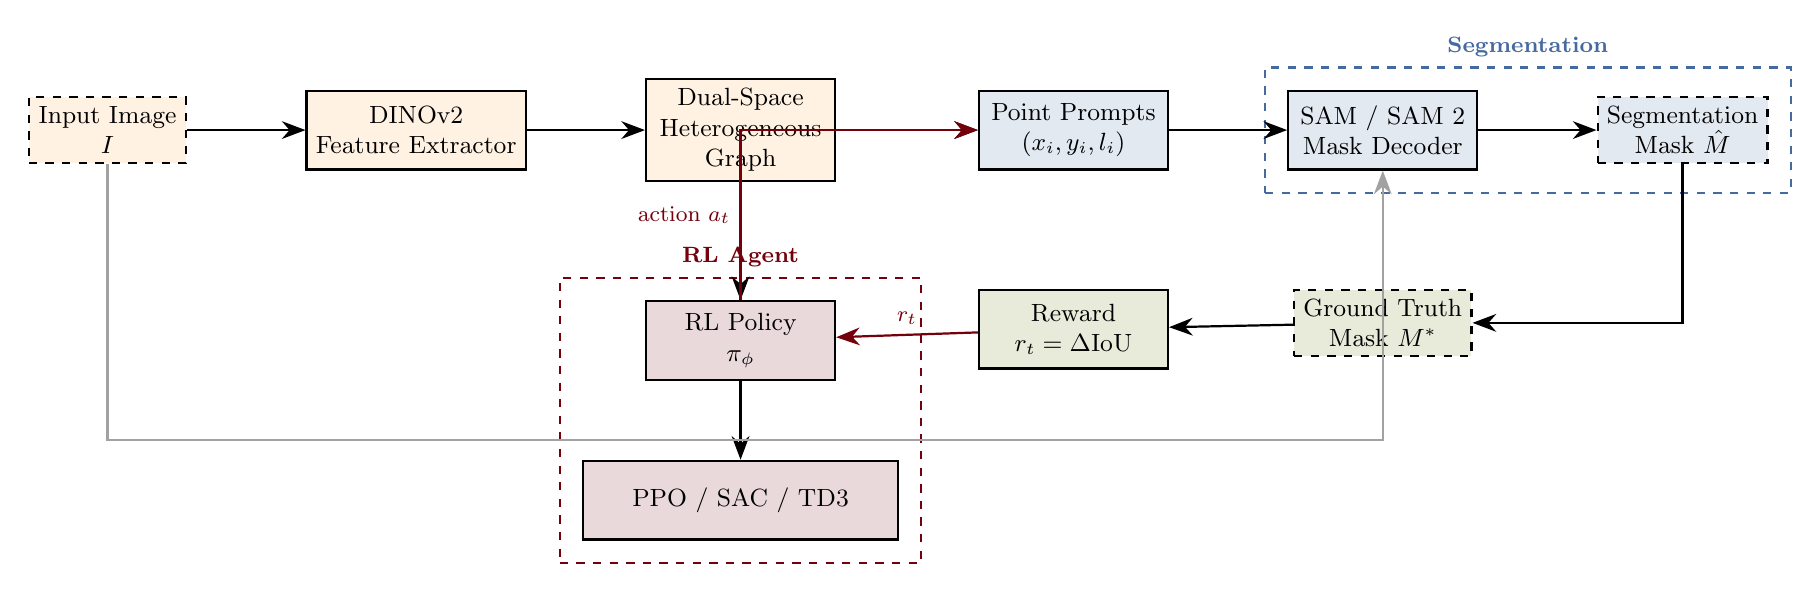
\begin{tikzpicture}[
    block/.style={draw, thick, minimum width=2.4cm, minimum height=1.0cm, align=center, font=\small},
    data/.style={draw, thick, minimum width=2.0cm, minimum height=0.8cm, align=center, font=\small, dashed},
    arr/.style={-{Stealth[length=3mm]}, thick},
    every node/.style={font=\small}
]

% Input Image
\node[data, fill=sandstorm] (img) {Input Image\\$I$};

% DINOv2
\node[block, fill=sandstorm, right=1.5cm of img] (dino) {DINOv2\\Feature Extractor};

% Dual-Space Graph
\node[block, fill=sandstorm, right=1.5cm of dino] (graph) {Dual-Space\\Heterogeneous\\Graph};

% RL Policy
\node[block, fill=garnet!15, below=1.5cm of graph] (policy) {RL Policy\\$\pi_\phi$};

% Algorithm choices
\node[block, fill=garnet!15, below=1.0cm of policy, minimum width=4.0cm] (algos) {PPO / SAC / TD3};

% Point Prompts
\node[block, fill=atlantic!15, right=1.8cm of graph] (prompts) {Point Prompts\\$(x_i, y_i, l_i)$};

% SAM / SAM 2
\node[block, fill=atlantic!15, right=1.5cm of prompts] (sam) {SAM / SAM 2\\Mask Decoder};

% Output Mask
\node[data, fill=atlantic!15, right=1.5cm of sam] (mask) {Segmentation\\Mask $\hat{M}$};

% Ground Truth
\node[data, fill=horseshoe!15, below=1.5cm of sam] (gt) {Ground Truth\\Mask $M^*$};

% Reward
\node[block, fill=horseshoe!15, below=1.5cm of prompts] (reward) {Reward\\$r_t = \Delta\text{IoU}$};

% Arrows
\draw[arr] (img) -- (dino);
\draw[arr] (dino) -- (graph);
\draw[arr] (graph) -- (prompts);
\draw[arr] (prompts) -- (sam);
\draw[arr] (sam) -- (mask);

% RL loop
\draw[arr] (graph) -- (policy);
\draw[arr, garnet] (policy) -- node[left, font=\footnotesize, text=garnet] {action $a_t$} (policy |- graph) -- (prompts);
\draw[arr] (mask) -- (mask |- gt) -- (gt);
\draw[arr] (gt) -- (reward);
\draw[arr, garnet] (reward) -- node[above, font=\footnotesize, text=garnet] {$r_t$} (policy);
\draw[arr] (policy) -- (algos);

% Image also to SAM
\draw[arr, black50] (img) |- ([yshift=-3.5cm]img.south) -| (sam.south);

% Background boxes
\begin{scope}[on background layer]
\node[draw=garnet, thick, dashed, inner sep=8pt, fit=(policy)(algos), label={[font=\footnotesize\bfseries, text=garnet]above:RL Agent}] {};
\node[draw=atlantic, thick, dashed, inner sep=8pt, fit=(sam)(mask), label={[font=\footnotesize\bfseries, text=atlantic]above:Segmentation}] {};
\end{scope}

\end{tikzpicture}
\caption{System architecture of the extended Plug-and-Play prompt optimization framework. An input image is processed by DINOv2 to construct a dual-space heterogeneous graph encoding feature similarity and spatial proximity. The RL policy (PPO, SAC, or TD3) selects point prompt coordinates and labels, which are passed to SAM or SAM 2 for mask generation. The segmentation quality improvement (IoU delta) serves as the reward signal, closing the optimization loop.}
\label{fig:system_arch}
\end{figure*}

% ============================================================
% APPROACH
% ============================================================
\section{Approach}

\subsection{Background: Plug-and-Play PPO}

The original Plug-and-Play PPO~\cite{Liu2025PlugAndPlayPPO} reformulates prompt optimization as a heterogeneous graph optimization problem solved via deep reinforcement learning. Given a reference image with a known mask and a target image, DINOv2~\cite{Oquab2024DINOv2} extracts patch-level features for both images. The system constructs a dual-space graph where nodes represent image patches and edges encode two types of relationships: \textit{feature similarity} in the DINOv2 embedding space and \textit{physical proximity} in pixel coordinates. This heterogeneous graph captures both semantic and spatial structure, enabling the policy to reason about which image regions are likely foreground versus background.

The RL agent operates over this graph representation. At each step $t$, the state $s_t$ consists of the graph encoding, the current segmentation mask, and the set of previously placed prompts. The action $a_t$ specifies a point coordinate $(x, y)$ and a label $l \in \{+1, -1\}$ indicating a positive (foreground) or negative (background) prompt. The reward $r_t$ is the change in Intersection-over-Union (IoU) between the predicted mask and ground truth after the new prompt is applied. The policy is trained with PPO~\cite{Schulman2017PPO} to maximize cumulative IoU improvement across iterative prompt refinement steps.

\subsection{Extension 1: Algorithm Comparison}

PPO is an on-policy algorithm that discards collected experience after each policy update, which can limit sample efficiency in environments where each interaction is computationally expensive. We propose replacing PPO with two off-policy alternatives that maintain a replay buffer of past transitions.

\textit{Soft Actor-Critic} (SAC)~\cite{Haarnoja2018SAC} maximizes a maximum-entropy objective $J(\pi) = \sum_t \mathbb{E}_{(s_t, a_t) \sim \rho_\pi}\left[r(s_t, a_t) + \alpha \mathcal{H}(\pi(\cdot | s_t))\right]$, where $\alpha$ controls the entropy bonus $\mathcal{H}$. The entropy term encourages exploration of diverse prompt placements, which is particularly valuable in early training when the policy has not yet learned which regions are informative. SAC uses two Q-networks to mitigate overestimation bias and updates the policy via the reparameterization trick for continuous actions.

\textit{Twin Delayed DDPG} (TD3)~\cite{Fujimoto2018TD3} extends DDPG with three key modifications: clipped double Q-learning to reduce value overestimation, delayed policy updates to reduce per-update error, and target policy smoothing to prevent the policy from exploiting narrow peaks in the Q-function. TD3 uses a deterministic policy with additive exploration noise, contrasting with SAC's stochastic policy.

To enable continuous-valued point coordinate prediction with SAC and TD3, we parameterize the action space as $a_t = (x, y, p) \in [0, 1]^3$, where $(x, y)$ are normalized image coordinates and $p$ is thresholded to determine the prompt label ($l = +1$ if $p > 0.5$, else $l = -1$). For PPO, we retain the original discrete action formulation from~\cite{Liu2025PlugAndPlayPPO} for fair comparison.

% ============================================================
% FIGURE 2: MDP FORMULATION
% ============================================================
\begin{figure}[t]
\centering
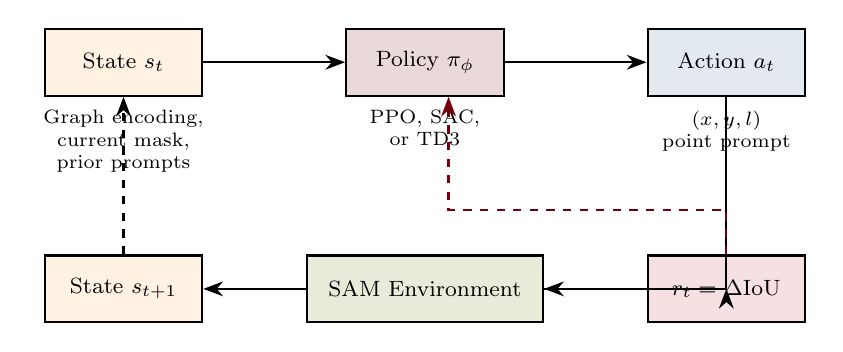
\begin{tikzpicture}[
    block/.style={draw, thick, minimum width=2.0cm, minimum height=0.85cm, align=center, font=\footnotesize},
    arr/.style={-{Stealth[length=2.5mm]}, thick},
    every node/.style={font=\footnotesize}
]

% State
\node[block, fill=sandstorm] (st) {State $s_t$};
\node[below=0.05cm of st, font=\scriptsize, text width=2.2cm, align=center] (stdetail) {Graph encoding,\\current mask,\\prior prompts};

% Policy
\node[block, fill=garnet!15, right=1.8cm of st] (pi) {Policy $\pi_\phi$};
\node[below=0.05cm of pi, font=\scriptsize, text width=2.0cm, align=center] (pidetail) {PPO, SAC,\\or TD3};

% Action
\node[block, fill=atlantic!15, right=1.8cm of pi] (at) {Action $a_t$};
\node[below=0.05cm of at, font=\scriptsize, text width=2.0cm, align=center] (atdetail) {$(x, y, l)$\\point prompt};

% Environment
\node[block, fill=horseshoe!15, below=2.0cm of pi, minimum width=3.0cm] (env) {SAM Environment};

% Next state
\node[block, fill=sandstorm, below=2.0cm of st] (st1) {State $s_{t+1}$};

% Reward
\node[block, fill=rose!15, below=2.0cm of at] (rt) {$r_t = \Delta\text{IoU}$};

% Arrows
\draw[arr] (st) -- (pi);
\draw[arr] (pi) -- (at);
\draw[arr] (at) |- (env);
\draw[arr] (env) -- (st1);
\draw[arr] (env) -| (rt);
\draw[arr, dashed] (st1) -- (st);
\draw[arr, garnet, dashed] (rt) -- ++(0, 1.0) -| ([xshift=0.3cm]pi.south);

\end{tikzpicture}
\caption{MDP formulation for RL-based prompt optimization. The state encodes the dual-space graph, current mask, and prior prompts. The policy selects point coordinates and labels. SAM produces a new mask, and the IoU improvement serves as the reward.}
\label{fig:mdp}
\end{figure}

\subsection{Extension 2: Domain Transfer}

A key claim of SAM is zero-shot generalizability across visual domains. However, prompt sensitivity varies dramatically across domains. Medical images exhibit low contrast and ambiguous boundaries~\cite{Zhang2024MedSAM}, while remote sensing imagery contains densely packed objects at multiple scales~\cite{Osco2023SAMRemoteSensing}. We evaluate whether a prompt optimizer trained on natural images (Pascal VOC~\cite{Everingham2010VOC}) transfers to these specialized domains, and whether domain-specific fine-tuning of the RL policy improves results. AlignSAM~\cite{Huang2024AlignSAM} demonstrated that RL can align SAM to open-context scenarios via reinforcement learning from human feedback, motivating our hypothesis that RL-based prompt optimization can similarly adapt across domains.

\subsection{Extension 3: Temporal Prompting with SAM 2}

SAM 2~\cite{Ravi2024SAM2} extends the original SAM architecture to video with a memory-augmented streaming design. A memory bank stores spatial features and object pointers from previous frames, and a memory attention module conditions the current frame's features on this temporal context. SAM 2 achieves state-of-the-art video object segmentation while running at approximately 44 frames per second. Recent work on SAM2RL~\cite{Yang2025SAM2RL} demonstrates that RL can optimize SAM 2's memory bank management, achieving improvements exceeding three times the gains of hand-crafted heuristics.

We propose adapting the prompt optimizer for video input by augmenting the state representation with temporal features. At frame $t$, the state includes not only the current frame's dual-space graph but also a summary of the previous frame's mask and prompt history. The reward is modified to include a temporal consistency term $r_t = \Delta\text{IoU}_t + \beta \cdot \text{TC}_t$, where $\text{TC}_t$ measures the smoothness of mask boundaries across consecutive frames. This encourages the policy to select prompts that maintain stable object tracking rather than optimizing each frame independently.

% ============================================================
% FIGURE 3: SAM 2 TEMPORAL EXTENSION
% ============================================================
\begin{figure}[t]
\centering
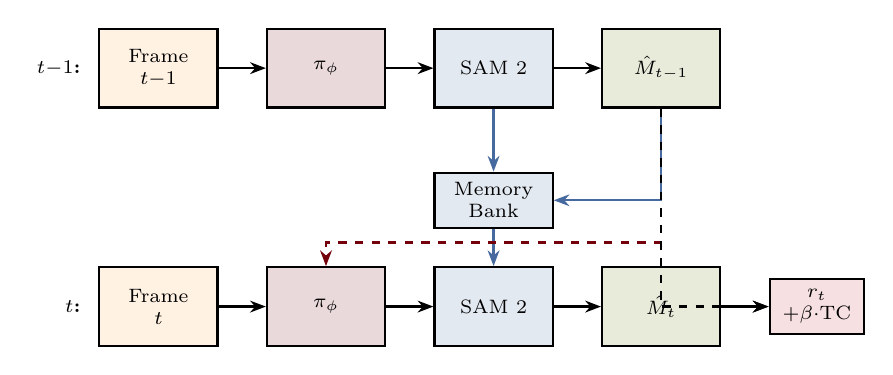
\begin{tikzpicture}[
    frame/.style={draw, thick, minimum width=1.5cm, minimum height=1.0cm, align=center, font=\scriptsize},
    mem/.style={draw, thick, minimum width=1.5cm, minimum height=0.7cm, align=center, font=\scriptsize, fill=atlantic!15},
    arr/.style={-{Stealth[length=2mm]}, thick},
    every node/.style={font=\scriptsize}
]

% Frame t-1
\node[frame, fill=sandstorm] (f1) {Frame\\$t{-}1$};
\node[frame, fill=garnet!15, right=0.6cm of f1] (p1) {$\pi_\phi$};
\node[frame, fill=atlantic!15, right=0.6cm of p1] (s1) {SAM 2};
\node[frame, fill=horseshoe!15, right=0.6cm of s1] (m1) {$\hat{M}_{t-1}$};

% Memory
\node[mem, below=0.8cm of s1] (mem) {Memory\\Bank};

% Frame t
\node[frame, fill=sandstorm, below=2.0cm of f1] (f2) {Frame\\$t$};
\node[frame, fill=garnet!15, right=0.6cm of f2] (p2) {$\pi_\phi$};
\node[frame, fill=atlantic!15, right=0.6cm of p2] (s2) {SAM 2};
\node[frame, fill=horseshoe!15, right=0.6cm of s2] (m2) {$\hat{M}_{t}$};

% Arrows within frames
\draw[arr] (f1) -- (p1);
\draw[arr] (p1) -- (s1);
\draw[arr] (s1) -- (m1);
\draw[arr] (f2) -- (p2);
\draw[arr] (p2) -- (s2);
\draw[arr] (s2) -- (m2);

% Memory connections
\draw[arr, atlantic] (s1) -- (mem);
\draw[arr, atlantic] (m1) |- (mem);
\draw[arr, atlantic] (mem) -- (s2);
\draw[arr, garnet, dashed] (m1) |- ([yshift=0.3cm]p2.north) -- (p2.north);

% TC reward
\node[draw, thick, fill=rose!15, right=0.6cm of m2, minimum width=1.2cm, minimum height=0.7cm, align=center] (tc) {$r_t$\\$+\beta\cdot$TC};
\draw[arr] (m2) -- (tc);
\draw[arr, dashed] (m1) |- (tc);

% Labels
\node[left=0.1cm of f1, font=\scriptsize\bfseries] {$t{-}1$:};
\node[left=0.1cm of f2, font=\scriptsize\bfseries] {$t$:};

\end{tikzpicture}
\caption{Temporal prompt optimization with SAM 2. The RL policy receives temporal context from previous frames via the memory bank and prior mask history. The reward includes a temporal consistency (TC) bonus to encourage smooth mask predictions across frames.}
\label{fig:sam2_temporal}
\end{figure}

\subsection{Extension 4: Boundary-Weighted Reward Shaping}

Standard IoU treats all pixels equally, which can underweight boundary accuracy for objects with thin protrusions or irregular edges. Following principles from reward shaping~\cite{Ng1999RewardShaping}, we propose a boundary-weighted IoU reward. Let $B^*$ denote the set of boundary pixels in the ground truth mask (obtained via morphological gradient) and $\hat{B}$ the corresponding boundary in the predicted mask. The shaped reward is defined as
\begin{align}
r_t^{\text{shaped}} = \Delta\text{IoU}_t + \gamma \cdot \Delta\text{BIoU}_t
\label{eq:boundary_reward}
\end{align}
where $\text{BIoU}$ computes IoU restricted to a narrow band around object boundaries and $\gamma$ controls the boundary emphasis. For class-imbalanced datasets such as KVASIR-SEG where polyps vary dramatically in size, we additionally weight the reward inversely proportional to object area, preventing the policy from ignoring small objects.

% ============================================================
% FIGURE 4: ALGORITHM COMPARISON DIAGRAM
% ============================================================
\begin{figure}[t]
\centering
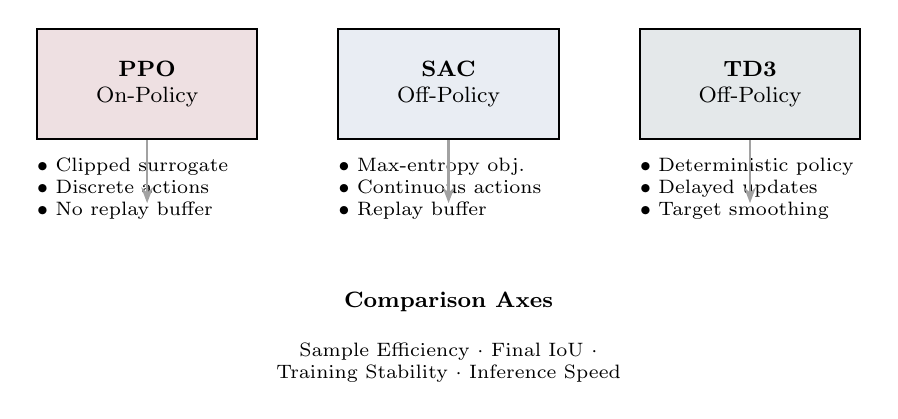
\begin{tikzpicture}[
    alg/.style={draw, thick, minimum width=2.8cm, minimum height=1.4cm, align=center, font=\footnotesize},
    prop/.style={font=\scriptsize, text width=2.8cm, align=left},
    arr/.style={-{Stealth[length=2mm]}, thick},
    every node/.style={font=\footnotesize}
]

% PPO
\node[alg, fill=garnet!12] (ppo) {\textbf{PPO}\\On-Policy};
\node[prop, below=0.1cm of ppo] (ppop) {
    $\bullet$ Clipped surrogate\\
    $\bullet$ Discrete actions\\
    $\bullet$ No replay buffer
};

% SAC
\node[alg, fill=atlantic!12, right=1.0cm of ppo] (sac) {\textbf{SAC}\\Off-Policy};
\node[prop, below=0.1cm of sac] (sacp) {
    $\bullet$ Max-entropy obj.\\
    $\bullet$ Continuous actions\\
    $\bullet$ Replay buffer
};

% TD3
\node[alg, fill=congaree!12, right=1.0cm of sac] (td3) {\textbf{TD3}\\Off-Policy};
\node[prop, below=0.1cm of td3] (td3p) {
    $\bullet$ Deterministic policy\\
    $\bullet$ Delayed updates\\
    $\bullet$ Target smoothing
};

% Comparison arrows
\node[below=1.8cm of sac, font=\footnotesize\bfseries] (comp) {Comparison Axes};
\node[below=0.15cm of comp, font=\scriptsize, text width=7cm, align=center] {
    Sample Efficiency $\cdot$ Final IoU $\cdot$ Training Stability $\cdot$ Inference Speed
};

\draw[arr, black50] (ppo.south) -- ++(0, -0.8);
\draw[arr, black50] (sac.south) -- ++(0, -0.8);
\draw[arr, black50] (td3.south) -- ++(0, -0.8);

\end{tikzpicture}
\caption{Comparison of three RL algorithms for prompt optimization. PPO (baseline from~\cite{Liu2025PlugAndPlayPPO}) operates on-policy with discrete actions. SAC and TD3 are off-policy with continuous action spaces and replay buffers, potentially offering improved sample efficiency.}
\label{fig:algo_comparison}
\end{figure}

% ============================================================
% EVALUATION
% ============================================================
\section{Evaluation}

\subsection{Datasets}

We evaluate on four datasets spanning diverse visual domains. Pascal VOC~\cite{Everingham2010VOC} provides 1,464 training and 1,449 validation images with 20 object categories, serving as the primary natural-image benchmark. FSS-1000~\cite{Li2020FSS1000} contains 1,000 classes with 10 images per class for few-shot segmentation evaluation. KVASIR-SEG~\cite{Jha2020KvasirSEG} provides 1,000 gastrointestinal polyp images for medical domain transfer evaluation. For video segmentation, we use the DAVIS 2017 benchmark, which contains 90 video sequences with dense per-frame annotations.

\subsection{Baselines}

We compare our extended methods against six baselines. \textit{Center-of-mass prompts} place a single positive point at the centroid of a coarse initial mask. \textit{Random point prompts} sample points uniformly from the image. \textit{Grid-based prompts} place points on a regular grid with labels assigned by a coarse mask. \textit{Original PPO}~\cite{Liu2025PlugAndPlayPPO} provides the direct replication baseline. \textit{Greedy heuristic} selects the point that maximizes instantaneous IoU at each step via exhaustive search over a candidate set. \textit{FocalClick}~\cite{Chen2022FocalClick} represents the supervised interactive segmentation baseline, and \textit{RITM}~\cite{Sofiiuk2022RITM} provides an iterative training baseline.

% ============================================================
% TABLE 1: EVALUATION PLAN
% ============================================================
\begin{table}[t]
\centering
\caption{Evaluation plan across datasets and proposed extensions.}
\label{tab:eval_plan}
\begin{tabular}{@{}lcccc@{}}
\toprule
\textbf{Dataset} & \textbf{Algo.} & \textbf{Domain} & \textbf{Video} & \textbf{Reward} \\
\midrule
Pascal VOC  & \checkmark & ---        & ---        & \checkmark \\
FSS-1000    & \checkmark & ---        & ---        & \checkmark \\
KVASIR-SEG  & \checkmark & \checkmark & ---        & \checkmark \\
DAVIS 2017  & \checkmark & ---        & \checkmark & \checkmark \\
\bottomrule
\end{tabular}
\end{table}

\subsection{Metrics}

The primary segmentation quality metrics are Intersection-over-Union (IoU) and Dice coefficient, reported as mean values across test images. We additionally report Boundary IoU (BIoU) to assess edge quality, the number of prompt iterations required to reach a target IoU threshold (efficiency), and wall-clock inference time per image. For the algorithm comparison, we measure sample efficiency as the number of environment interactions required to reach 90\% of final performance, and training stability as the variance of IoU across five random seeds. For video segmentation, we report the $\mathcal{J}\&\mathcal{F}$ metric (mean of region similarity $\mathcal{J}$ and contour accuracy $\mathcal{F}$) following standard VOS evaluation protocol.

\subsection{Ablation Studies}

We conduct the following ablations to isolate contributions of each component. Removing the dual-space graph and using raw image features as state measures the value of the heterogeneous graph encoding. Removing the boundary-weighted reward term measures the effect of reward shaping on boundary quality. For the video extension, removing the temporal consistency bonus measures whether temporal awareness improves tracking stability. Varying the entropy coefficient $\alpha$ in SAC and the exploration noise scale in TD3 quantifies the sensitivity of each algorithm to exploration hyperparameters.

% ============================================================
% FIGURE 5: EVALUATION PIPELINE
% ============================================================
\begin{figure}[t]
\centering
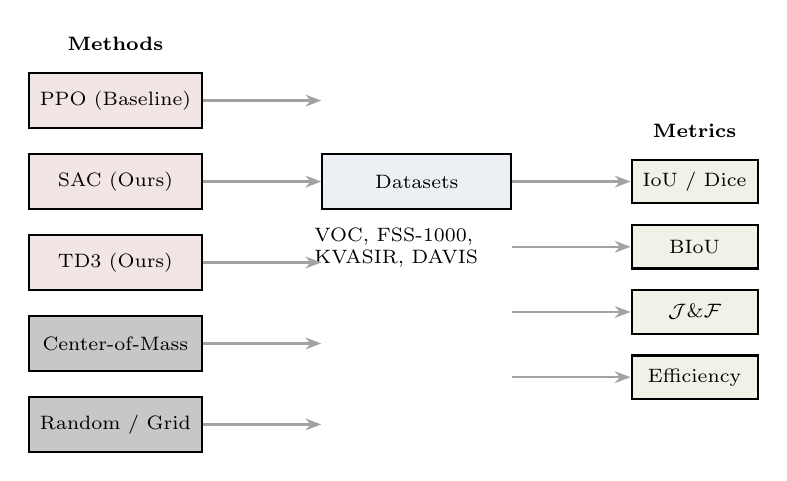
\begin{tikzpicture}[
    block/.style={draw, thick, minimum width=2.2cm, minimum height=0.7cm, align=center, font=\scriptsize},
    metric/.style={draw, thick, minimum width=1.6cm, minimum height=0.55cm, align=center, font=\scriptsize, fill=white},
    arr/.style={-{Stealth[length=2mm]}, thick},
    every node/.style={font=\scriptsize}
]

% Methods column
\node[block, fill=garnet!10] (m1) {PPO (Baseline)};
\node[block, fill=garnet!10, below=0.3cm of m1] (m2) {SAC (Ours)};
\node[block, fill=garnet!10, below=0.3cm of m2] (m3) {TD3 (Ours)};
\node[block, fill=black30, below=0.3cm of m3] (m4) {Center-of-Mass};
\node[block, fill=black30, below=0.3cm of m4] (m5) {Random / Grid};

% Datasets
\node[block, fill=atlantic!10, right=1.5cm of m2, minimum width=2.4cm] (ds) {Datasets};
\node[below=0.1cm of ds, font=\scriptsize, text width=2.6cm, align=left] (dslist) {
    VOC, FSS-1000,\\
    KVASIR, DAVIS
};

% Metrics
\node[metric, fill=horseshoe!10, right=1.5cm of ds] (met1) {IoU / Dice};
\node[metric, fill=horseshoe!10, below=0.25cm of met1] (met2) {BIoU};
\node[metric, fill=horseshoe!10, below=0.25cm of met2] (met3) {$\mathcal{J}\&\mathcal{F}$};
\node[metric, fill=horseshoe!10, below=0.25cm of met3] (met4) {Efficiency};

% Arrows
\foreach \m in {m1,m2,m3,m4,m5} {
    \draw[arr, black50] (\m.east) -- (ds.west |- \m);
}
\draw[arr, black50] (ds.east |- met1) -- (met1.west);
\draw[arr, black50] (ds.east |- met2) -- (met2.west);
\draw[arr, black50] (ds.east |- met3) -- (met3.west);
\draw[arr, black50] (ds.east |- met4) -- (met4.west);

% Labels
\node[above=0.15cm of m1, font=\scriptsize\bfseries] {Methods};
\node[above=0.15cm of met1, font=\scriptsize\bfseries] {Metrics};

\end{tikzpicture}
\caption{Evaluation pipeline. RL-based methods (PPO, SAC, TD3) and non-RL baselines are evaluated across four datasets using segmentation quality, boundary accuracy, video tracking, and prompt efficiency metrics.}
\label{fig:eval_pipeline}
\end{figure}

% ============================================================
% TABLE 2: EXPECTED COMPARISON
% ============================================================
\begin{table}[t]
\centering
\caption{Expected algorithmic properties of each RL method.}
\label{tab:algo_properties}
\begin{tabular}{@{}lccc@{}}
\toprule
\textbf{Property} & \textbf{PPO} & \textbf{SAC} & \textbf{TD3} \\
\midrule
Policy Type         & Stochastic & Stochastic & Deterministic \\
On/Off-Policy       & On-policy  & Off-policy & Off-policy \\
Action Space        & Discrete   & Continuous & Continuous \\
Replay Buffer       & No         & Yes        & Yes \\
Entropy Bonus       & No         & Yes        & No \\
Sample Efficiency   & Low        & High       & High \\
\bottomrule
\end{tabular}
\end{table}

% ============================================================
% CONCLUSION
% ============================================================
\section{Conclusion}

We propose to replicate and extend the Plug-and-Play PPO framework for RL-based point prompt optimization in SAM segmentation. Our extensions span four complementary directions: comparing PPO against off-policy alternatives (SAC and TD3) for prompt coordinate prediction, evaluating domain transfer to medical and remote sensing imagery, adapting the prompt optimizer for temporally consistent video segmentation with SAM 2, and introducing boundary-weighted reward shaping to improve mask quality on challenging structures. The evaluation plan covers four datasets (Pascal VOC, FSS-1000, KVASIR-SEG, DAVIS 2017), seven baselines, and five metric families, with ablation studies to isolate the contribution of each proposed component. This work will provide empirical evidence for whether off-policy RL algorithms can outperform PPO for prompt optimization, whether RL-trained prompt policies transfer across visual domains, and whether temporal awareness and shaped rewards yield measurable improvements in segmentation quality. The project leverages an existing published codebase~\cite{Liu2025PlugAndPlayPPO} with standard benchmarks, providing a low-risk foundation for these novel extensions.

% ============================================================
% REFERENCES
% ============================================================
\bibliographystyle{IEEEtran}
\bibliography{references}
\nocite{*}

\end{document}
